\documentclass{article} % For LaTeX2e
\usepackage{iclr2027_conference,times}

% Optional math commands from https://github.com/goodfeli/dlbook_notation.
%%%%% NEW MATH DEFINITIONS %%%%%

\usepackage{amsmath,amsfonts,bm}

% Mark sections of captions for referring to divisions of figures
\newcommand{\figleft}{{\em (Left)}}
\newcommand{\figcenter}{{\em (Center)}}
\newcommand{\figright}{{\em (Right)}}
\newcommand{\figtop}{{\em (Top)}}
\newcommand{\figbottom}{{\em (Bottom)}}
\newcommand{\captiona}{{\em (a)}}
\newcommand{\captionb}{{\em (b)}}
\newcommand{\captionc}{{\em (c)}}
\newcommand{\captiond}{{\em (d)}}

% Highlight a newly defined term
\newcommand{\newterm}[1]{{\bf #1}}


% Figure reference, lower-case.
\def\figref#1{figure~\ref{#1}}
% Figure reference, capital. For start of sentence
\def\Figref#1{Figure~\ref{#1}}
\def\twofigref#1#2{figures \ref{#1} and \ref{#2}}
\def\quadfigref#1#2#3#4{figures \ref{#1}, \ref{#2}, \ref{#3} and \ref{#4}}
% Section reference, lower-case.
\def\secref#1{section~\ref{#1}}
% Section reference, capital.
\def\Secref#1{Section~\ref{#1}}
% Reference to two sections.
\def\twosecrefs#1#2{sections \ref{#1} and \ref{#2}}
% Reference to three sections.
\def\secrefs#1#2#3{sections \ref{#1}, \ref{#2} and \ref{#3}}
% Reference to an equation, lower-case.
\def\eqref#1{equation~\ref{#1}}
% Reference to an equation, upper case
\def\Eqref#1{Equation~\ref{#1}}
% A raw reference to an equation---avoid using if possible
\def\plaineqref#1{\ref{#1}}
% Reference to a chapter, lower-case.
\def\chapref#1{chapter~\ref{#1}}
% Reference to an equation, upper case.
\def\Chapref#1{Chapter~\ref{#1}}
% Reference to a range of chapters
\def\rangechapref#1#2{chapters\ref{#1}--\ref{#2}}
% Reference to an algorithm, lower-case.
\def\algref#1{algorithm~\ref{#1}}
% Reference to an algorithm, upper case.
\def\Algref#1{Algorithm~\ref{#1}}
\def\twoalgref#1#2{algorithms \ref{#1} and \ref{#2}}
\def\Twoalgref#1#2{Algorithms \ref{#1} and \ref{#2}}
% Reference to a part, lower case
\def\partref#1{part~\ref{#1}}
% Reference to a part, upper case
\def\Partref#1{Part~\ref{#1}}
\def\twopartref#1#2{parts \ref{#1} and \ref{#2}}

\def\ceil#1{\lceil #1 \rceil}
\def\floor#1{\lfloor #1 \rfloor}
\def\1{\bm{1}}
\newcommand{\train}{\mathcal{D}}
\newcommand{\valid}{\mathcal{D_{\mathrm{valid}}}}
\newcommand{\test}{\mathcal{D_{\mathrm{test}}}}

\def\eps{{\epsilon}}


% Random variables
\def\reta{{\textnormal{$\eta$}}}
\def\ra{{\textnormal{a}}}
\def\rb{{\textnormal{b}}}
\def\rc{{\textnormal{c}}}
\def\rd{{\textnormal{d}}}
\def\re{{\textnormal{e}}}
\def\rf{{\textnormal{f}}}
\def\rg{{\textnormal{g}}}
\def\rh{{\textnormal{h}}}
\def\ri{{\textnormal{i}}}
\def\rj{{\textnormal{j}}}
\def\rk{{\textnormal{k}}}
\def\rl{{\textnormal{l}}}
% rm is already a command, just don't name any random variables m
\def\rn{{\textnormal{n}}}
\def\ro{{\textnormal{o}}}
\def\rp{{\textnormal{p}}}
\def\rq{{\textnormal{q}}}
\def\rr{{\textnormal{r}}}
\def\rs{{\textnormal{s}}}
\def\rt{{\textnormal{t}}}
\def\ru{{\textnormal{u}}}
\def\rv{{\textnormal{v}}}
\def\rw{{\textnormal{w}}}
\def\rx{{\textnormal{x}}}
\def\ry{{\textnormal{y}}}
\def\rz{{\textnormal{z}}}

% Random vectors
\def\rvepsilon{{\mathbf{\epsilon}}}
\def\rvtheta{{\mathbf{\theta}}}
\def\rva{{\mathbf{a}}}
\def\rvb{{\mathbf{b}}}
\def\rvc{{\mathbf{c}}}
\def\rvd{{\mathbf{d}}}
\def\rve{{\mathbf{e}}}
\def\rvf{{\mathbf{f}}}
\def\rvg{{\mathbf{g}}}
\def\rvh{{\mathbf{h}}}
\def\rvu{{\mathbf{i}}}
\def\rvj{{\mathbf{j}}}
\def\rvk{{\mathbf{k}}}
\def\rvl{{\mathbf{l}}}
\def\rvm{{\mathbf{m}}}
\def\rvn{{\mathbf{n}}}
\def\rvo{{\mathbf{o}}}
\def\rvp{{\mathbf{p}}}
\def\rvq{{\mathbf{q}}}
\def\rvr{{\mathbf{r}}}
\def\rvs{{\mathbf{s}}}
\def\rvt{{\mathbf{t}}}
\def\rvu{{\mathbf{u}}}
\def\rvv{{\mathbf{v}}}
\def\rvw{{\mathbf{w}}}
\def\rvx{{\mathbf{x}}}
\def\rvy{{\mathbf{y}}}
\def\rvz{{\mathbf{z}}}

% Elements of random vectors
\def\erva{{\textnormal{a}}}
\def\ervb{{\textnormal{b}}}
\def\ervc{{\textnormal{c}}}
\def\ervd{{\textnormal{d}}}
\def\erve{{\textnormal{e}}}
\def\ervf{{\textnormal{f}}}
\def\ervg{{\textnormal{g}}}
\def\ervh{{\textnormal{h}}}
\def\ervi{{\textnormal{i}}}
\def\ervj{{\textnormal{j}}}
\def\ervk{{\textnormal{k}}}
\def\ervl{{\textnormal{l}}}
\def\ervm{{\textnormal{m}}}
\def\ervn{{\textnormal{n}}}
\def\ervo{{\textnormal{o}}}
\def\ervp{{\textnormal{p}}}
\def\ervq{{\textnormal{q}}}
\def\ervr{{\textnormal{r}}}
\def\ervs{{\textnormal{s}}}
\def\ervt{{\textnormal{t}}}
\def\ervu{{\textnormal{u}}}
\def\ervv{{\textnormal{v}}}
\def\ervw{{\textnormal{w}}}
\def\ervx{{\textnormal{x}}}
\def\ervy{{\textnormal{y}}}
\def\ervz{{\textnormal{z}}}

% Random matrices
\def\rmA{{\mathbf{A}}}
\def\rmB{{\mathbf{B}}}
\def\rmC{{\mathbf{C}}}
\def\rmD{{\mathbf{D}}}
\def\rmE{{\mathbf{E}}}
\def\rmF{{\mathbf{F}}}
\def\rmG{{\mathbf{G}}}
\def\rmH{{\mathbf{H}}}
\def\rmI{{\mathbf{I}}}
\def\rmJ{{\mathbf{J}}}
\def\rmK{{\mathbf{K}}}
\def\rmL{{\mathbf{L}}}
\def\rmM{{\mathbf{M}}}
\def\rmN{{\mathbf{N}}}
\def\rmO{{\mathbf{O}}}
\def\rmP{{\mathbf{P}}}
\def\rmQ{{\mathbf{Q}}}
\def\rmR{{\mathbf{R}}}
\def\rmS{{\mathbf{S}}}
\def\rmT{{\mathbf{T}}}
\def\rmU{{\mathbf{U}}}
\def\rmV{{\mathbf{V}}}
\def\rmW{{\mathbf{W}}}
\def\rmX{{\mathbf{X}}}
\def\rmY{{\mathbf{Y}}}
\def\rmZ{{\mathbf{Z}}}

% Elements of random matrices
\def\ermA{{\textnormal{A}}}
\def\ermB{{\textnormal{B}}}
\def\ermC{{\textnormal{C}}}
\def\ermD{{\textnormal{D}}}
\def\ermE{{\textnormal{E}}}
\def\ermF{{\textnormal{F}}}
\def\ermG{{\textnormal{G}}}
\def\ermH{{\textnormal{H}}}
\def\ermI{{\textnormal{I}}}
\def\ermJ{{\textnormal{J}}}
\def\ermK{{\textnormal{K}}}
\def\ermL{{\textnormal{L}}}
\def\ermM{{\textnormal{M}}}
\def\ermN{{\textnormal{N}}}
\def\ermO{{\textnormal{O}}}
\def\ermP{{\textnormal{P}}}
\def\ermQ{{\textnormal{Q}}}
\def\ermR{{\textnormal{R}}}
\def\ermS{{\textnormal{S}}}
\def\ermT{{\textnormal{T}}}
\def\ermU{{\textnormal{U}}}
\def\ermV{{\textnormal{V}}}
\def\ermW{{\textnormal{W}}}
\def\ermX{{\textnormal{X}}}
\def\ermY{{\textnormal{Y}}}
\def\ermZ{{\textnormal{Z}}}

% Vectors
\def\vzero{{\bm{0}}}
\def\vone{{\bm{1}}}
\def\vmu{{\bm{\mu}}}
\def\vtheta{{\bm{\theta}}}
\def\va{{\bm{a}}}
\def\vb{{\bm{b}}}
\def\vc{{\bm{c}}}
\def\vd{{\bm{d}}}
\def\ve{{\bm{e}}}
\def\vf{{\bm{f}}}
\def\vg{{\bm{g}}}
\def\vh{{\bm{h}}}
\def\vi{{\bm{i}}}
\def\vj{{\bm{j}}}
\def\vk{{\bm{k}}}
\def\vl{{\bm{l}}}
\def\vm{{\bm{m}}}
\def\vn{{\bm{n}}}
\def\vo{{\bm{o}}}
\def\vp{{\bm{p}}}
\def\vq{{\bm{q}}}
\def\vr{{\bm{r}}}
\def\vs{{\bm{s}}}
\def\vt{{\bm{t}}}
\def\vu{{\bm{u}}}
\def\vv{{\bm{v}}}
\def\vw{{\bm{w}}}
\def\vx{{\bm{x}}}
\def\vy{{\bm{y}}}
\def\vz{{\bm{z}}}

% Elements of vectors
\def\evalpha{{\alpha}}
\def\evbeta{{\beta}}
\def\evepsilon{{\epsilon}}
\def\evlambda{{\lambda}}
\def\evomega{{\omega}}
\def\evmu{{\mu}}
\def\evpsi{{\psi}}
\def\evsigma{{\sigma}}
\def\evtheta{{\theta}}
\def\eva{{a}}
\def\evb{{b}}
\def\evc{{c}}
\def\evd{{d}}
\def\eve{{e}}
\def\evf{{f}}
\def\evg{{g}}
\def\evh{{h}}
\def\evi{{i}}
\def\evj{{j}}
\def\evk{{k}}
\def\evl{{l}}
\def\evm{{m}}
\def\evn{{n}}
\def\evo{{o}}
\def\evp{{p}}
\def\evq{{q}}
\def\evr{{r}}
\def\evs{{s}}
\def\evt{{t}}
\def\evu{{u}}
\def\evv{{v}}
\def\evw{{w}}
\def\evx{{x}}
\def\evy{{y}}
\def\evz{{z}}

% Matrix
\def\mA{{\bm{A}}}
\def\mB{{\bm{B}}}
\def\mC{{\bm{C}}}
\def\mD{{\bm{D}}}
\def\mE{{\bm{E}}}
\def\mF{{\bm{F}}}
\def\mG{{\bm{G}}}
\def\mH{{\bm{H}}}
\def\mI{{\bm{I}}}
\def\mJ{{\bm{J}}}
\def\mK{{\bm{K}}}
\def\mL{{\bm{L}}}
\def\mM{{\bm{M}}}
\def\mN{{\bm{N}}}
\def\mO{{\bm{O}}}
\def\mP{{\bm{P}}}
\def\mQ{{\bm{Q}}}
\def\mR{{\bm{R}}}
\def\mS{{\bm{S}}}
\def\mT{{\bm{T}}}
\def\mU{{\bm{U}}}
\def\mV{{\bm{V}}}
\def\mW{{\bm{W}}}
\def\mX{{\bm{X}}}
\def\mY{{\bm{Y}}}
\def\mZ{{\bm{Z}}}
\def\mBeta{{\bm{\beta}}}
\def\mPhi{{\bm{\Phi}}}
\def\mLambda{{\bm{\Lambda}}}
\def\mSigma{{\bm{\Sigma}}}

% Tensor
\DeclareMathAlphabet{\mathsfit}{\encodingdefault}{\sfdefault}{m}{sl}
\SetMathAlphabet{\mathsfit}{bold}{\encodingdefault}{\sfdefault}{bx}{n}
\newcommand{\tens}[1]{\bm{\mathsfit{#1}}}
\def\tA{{\tens{A}}}
\def\tB{{\tens{B}}}
\def\tC{{\tens{C}}}
\def\tD{{\tens{D}}}
\def\tE{{\tens{E}}}
\def\tF{{\tens{F}}}
\def\tG{{\tens{G}}}
\def\tH{{\tens{H}}}
\def\tI{{\tens{I}}}
\def\tJ{{\tens{J}}}
\def\tK{{\tens{K}}}
\def\tL{{\tens{L}}}
\def\tM{{\tens{M}}}
\def\tN{{\tens{N}}}
\def\tO{{\tens{O}}}
\def\tP{{\tens{P}}}
\def\tQ{{\tens{Q}}}
\def\tR{{\tens{R}}}
\def\tS{{\tens{S}}}
\def\tT{{\tens{T}}}
\def\tU{{\tens{U}}}
\def\tV{{\tens{V}}}
\def\tW{{\tens{W}}}
\def\tX{{\tens{X}}}
\def\tY{{\tens{Y}}}
\def\tZ{{\tens{Z}}}


% Graph
\def\gA{{\mathcal{A}}}
\def\gB{{\mathcal{B}}}
\def\gC{{\mathcal{C}}}
\def\gD{{\mathcal{D}}}
\def\gE{{\mathcal{E}}}
\def\gF{{\mathcal{F}}}
\def\gG{{\mathcal{G}}}
\def\gH{{\mathcal{H}}}
\def\gI{{\mathcal{I}}}
\def\gJ{{\mathcal{J}}}
\def\gK{{\mathcal{K}}}
\def\gL{{\mathcal{L}}}
\def\gM{{\mathcal{M}}}
\def\gN{{\mathcal{N}}}
\def\gO{{\mathcal{O}}}
\def\gP{{\mathcal{P}}}
\def\gQ{{\mathcal{Q}}}
\def\gR{{\mathcal{R}}}
\def\gS{{\mathcal{S}}}
\def\gT{{\mathcal{T}}}
\def\gU{{\mathcal{U}}}
\def\gV{{\mathcal{V}}}
\def\gW{{\mathcal{W}}}
\def\gX{{\mathcal{X}}}
\def\gY{{\mathcal{Y}}}
\def\gZ{{\mathcal{Z}}}

% Sets
\def\sA{{\mathbb{A}}}
\def\sB{{\mathbb{B}}}
\def\sC{{\mathbb{C}}}
\def\sD{{\mathbb{D}}}
% Don't use a set called E, because this would be the same as our symbol
% for expectation.
\def\sF{{\mathbb{F}}}
\def\sG{{\mathbb{G}}}
\def\sH{{\mathbb{H}}}
\def\sI{{\mathbb{I}}}
\def\sJ{{\mathbb{J}}}
\def\sK{{\mathbb{K}}}
\def\sL{{\mathbb{L}}}
\def\sM{{\mathbb{M}}}
\def\sN{{\mathbb{N}}}
\def\sO{{\mathbb{O}}}
\def\sP{{\mathbb{P}}}
\def\sQ{{\mathbb{Q}}}
\def\sR{{\mathbb{R}}}
\def\sS{{\mathbb{S}}}
\def\sT{{\mathbb{T}}}
\def\sU{{\mathbb{U}}}
\def\sV{{\mathbb{V}}}
\def\sW{{\mathbb{W}}}
\def\sX{{\mathbb{X}}}
\def\sY{{\mathbb{Y}}}
\def\sZ{{\mathbb{Z}}}

% Entries of a matrix
\def\emLambda{{\Lambda}}
\def\emA{{A}}
\def\emB{{B}}
\def\emC{{C}}
\def\emD{{D}}
\def\emE{{E}}
\def\emF{{F}}
\def\emG{{G}}
\def\emH{{H}}
\def\emI{{I}}
\def\emJ{{J}}
\def\emK{{K}}
\def\emL{{L}}
\def\emM{{M}}
\def\emN{{N}}
\def\emO{{O}}
\def\emP{{P}}
\def\emQ{{Q}}
\def\emR{{R}}
\def\emS{{S}}
\def\emT{{T}}
\def\emU{{U}}
\def\emV{{V}}
\def\emW{{W}}
\def\emX{{X}}
\def\emY{{Y}}
\def\emZ{{Z}}
\def\emSigma{{\Sigma}}

% entries of a tensor
% Same font as tensor, without \bm wrapper
\newcommand{\etens}[1]{\mathsfit{#1}}
\def\etLambda{{\etens{\Lambda}}}
\def\etA{{\etens{A}}}
\def\etB{{\etens{B}}}
\def\etC{{\etens{C}}}
\def\etD{{\etens{D}}}
\def\etE{{\etens{E}}}
\def\etF{{\etens{F}}}
\def\etG{{\etens{G}}}
\def\etH{{\etens{H}}}
\def\etI{{\etens{I}}}
\def\etJ{{\etens{J}}}
\def\etK{{\etens{K}}}
\def\etL{{\etens{L}}}
\def\etM{{\etens{M}}}
\def\etN{{\etens{N}}}
\def\etO{{\etens{O}}}
\def\etP{{\etens{P}}}
\def\etQ{{\etens{Q}}}
\def\etR{{\etens{R}}}
\def\etS{{\etens{S}}}
\def\etT{{\etens{T}}}
\def\etU{{\etens{U}}}
\def\etV{{\etens{V}}}
\def\etW{{\etens{W}}}
\def\etX{{\etens{X}}}
\def\etY{{\etens{Y}}}
\def\etZ{{\etens{Z}}}

% The true underlying data generating distribution
\newcommand{\pdata}{p_{\rm{data}}}
% The empirical distribution defined by the training set
\newcommand{\ptrain}{\hat{p}_{\rm{data}}}
\newcommand{\Ptrain}{\hat{P}_{\rm{data}}}
% The model distribution
\newcommand{\pmodel}{p_{\rm{model}}}
\newcommand{\Pmodel}{P_{\rm{model}}}
\newcommand{\ptildemodel}{\tilde{p}_{\rm{model}}}
% Stochastic autoencoder distributions
\newcommand{\pencode}{p_{\rm{encoder}}}
\newcommand{\pdecode}{p_{\rm{decoder}}}
\newcommand{\precons}{p_{\rm{reconstruct}}}

\newcommand{\laplace}{\mathrm{Laplace}} % Laplace distribution

\newcommand{\E}{\mathbb{E}}
\newcommand{\Ls}{\mathcal{L}}
\newcommand{\R}{\mathbb{R}}
\newcommand{\emp}{\tilde{p}}
\newcommand{\lr}{\alpha}
\newcommand{\reg}{\lambda}
\newcommand{\rect}{\mathrm{rectifier}}
\newcommand{\softmax}{\mathrm{softmax}}
\newcommand{\sigmoid}{\sigma}
\newcommand{\softplus}{\zeta}
\newcommand{\KL}{D_{\mathrm{KL}}}
\newcommand{\Var}{\mathrm{Var}}
\newcommand{\standarderror}{\mathrm{SE}}
\newcommand{\Cov}{\mathrm{Cov}}
% Wolfram Mathworld says $L^2$ is for function spaces and $\ell^2$ is for vectors
% But then they seem to use $L^2$ for vectors throughout the site, and so does
% wikipedia.
\newcommand{\normlzero}{L^0}
\newcommand{\normlone}{L^1}
\newcommand{\normltwo}{L^2}
\newcommand{\normlp}{L^p}
\newcommand{\normmax}{L^\infty}

\newcommand{\parents}{Pa} % See usage in notation.tex. Chosen to match Daphne's book.

\DeclareMathOperator*{\argmax}{arg\,max}
\DeclareMathOperator*{\argmin}{arg\,min}

\DeclareMathOperator{\sign}{sign}
\DeclareMathOperator{\Tr}{Tr}
\let\ab\allowbreak


\usepackage{hyperref}
\usepackage{url}
\usepackage{booktabs}
\usepackage{graphicx}
\usepackage{wrapfig}

\title{Whose Word Survives Compression?}

% Authors must not appear in the submitted version. They should be hidden
% as long as the \iclrfinalcopy macro remains commented out below.
\author{Anonymous authors \\ Paper under double-blind review}

\newcommand{\fix}{\marginpar{FIX}}
\newcommand{\new}{\marginpar{NEW}}

%\iclrfinalcopy % Uncomment for camera-ready version, but NOT for submission.
\begin{document}

\maketitle

\begin{abstract}
Post-training quantization can preserve answer accuracy while changing the computation that selects between retrieved context and parametric memory. We test this possibility with JuICE, a dual-run attention-head intervention, on Llama-3.1-8B and Gemma-2-9B base models under GPTQ INT4. We identify source-arbitration heads on FP16, lock them, and test forward transfer, random-head controls, and in-precision application on 50 held-out conflict items. On Llama, an FP16 context-head set transfers head-specifically to INT4 ($+18$ percentage points (pp), 95\% CI $[+8,+30]$); the FP16 parametric intervention is not detected after quantization despite multiple recovery attempts. On Gemma, the directional ranking misses the raw positive parametric peak: steering that single head transfers head-specifically from $-12$ pp $[-22,-4]$ on FP16 to $-8$ pp $[-16,-2]$ on INT4, whereas a random-head control is exactly zero. The same ranking blind spot appears in both families. A Gemma context-suppression effect is detected at both precisions but is not distinguishable from its locked random-$K$ control, illustrating why intervention efficacy alone is insufficient evidence of circuit transfer. Thus, quantization transfer is neither uniformly preserved nor determined by source category; circuit-level claims require direct controls of intervention specificity.
\end{abstract}

\section{Introduction}
\label{sec:intro}

When retrieved context contradicts a model's parametric memory, a small set of attention heads can be used, at test time, to steer whose word the model trusts \citep{li2025taming}. This paper asks whether that residual-stream geometry is an FP16 object or a property of the model that survives compression: if JuICE is computed on FP16, does it still steer after GPTQ INT4, even on items whose facts survive quantization? Accuracy can fall from forgetting, terse decoding, or a change in source arbitration; a transferred intervention distinguishes those cases. Figure~\ref{fig:overview} is the test: identify causal heads on FP16, verify them by dual-run steering, then apply the locked heads to GPTQ INT4, on Llama-3.1-8B and Gemma-2-9B base \citep{grattafiori2024llama,team2024gemma2}, after a behavioral check on Llama Instruct.

\begin{figure}[!ht]
\centering
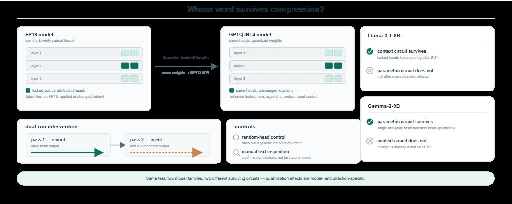
\includegraphics[width=\linewidth]{paper_overview_figure.pdf}
\caption{Experimental pipeline. FP16 identifies and locks causal heads, which transfer unchanged to a GPTQ INT4 model through a dual-run intervention (pass 1 records; pass 2 injects). Random-head control and manual text inspection support the outcome panels: Llama-3.1-8B retains the context circuit but not the parametric circuit, whereas Gemma-2-9B retains a parametric circuit but not the context circuit.}
\label{fig:overview}
\end{figure}

The contribution is a causal, head-level transfer test under GPTQ INT4 \citep{frantar2023gptq}, not a new accuracy table. Two objects transfer head-specifically---Llama context K10 and Gemma's raw parametric peak---but neither source category predicts transfer, and a detected Gemma context-suppression effect is not distinguishable from a locked random-head control. Behavioral efficacy is not, by itself, evidence that the same causal object survived compression.

Concretely, we show:
\begin{enumerate}
\item On Llama-3.1-8B-Instruct, GPTQ INT4 preserves closed-book recall on a double-filtered set while shifting conflict arbitration toward context (MR$^\star$ $-23.8$~pp $[-31.7,-17.1]$; cluster-robust AME $+10.3$~pp $[+3.1,+17.5]$).
\item On Llama-3.1-8B base, FP16 context K10 transfers head-specifically to INT4 ($+18$ $[+8,+30]$ vs.\ random-K10 $-6$ $[-14,0]$) and is recovered by native INT4 identification. Reverse transfer is a scorer artifact, not the same circuit. Parametric JuICE is a detected FP16 effect and a null at $\alpha{=}1$ on INT4 after rescale, raw-peak, native re-ID, and suppression repairs.
\item On Gemma-2-9B base, directional ranking again buries the raw parametric peak. Steering that peak (L27\_H6) transfers head-specifically ($-12$ $[-22,-4]$ on FP16; $-8$ $[-16,-2]$ on INT4; random-$K{=}1$ exactly $0$). Context K10 enlarge is a ceiling null; context suppression is detected at both precisions but its identified-versus-random contrast, and the difference-in-differences, include 0.
\item The transferable object is therefore family-specific. Quantization-selectivity is not a universal ``context lives / parametric dies'' rule.
\end{enumerate}

\section{Related Work}
\label{sec:related}

When retrieved context contradicts parametric memory, a language model must decide whose word to trust \citep{xie2024adaptive}. JuICE \citep{li2025taming} is a test-time, training-free dual-run intervention on a small set of attention heads. The original JuICE models are base checkpoints, not Instruct---a distinction that is load-bearing below (\S\ref{sec:instruct-base}). We do not revive a memory-head versus context-head dichotomy \citep{jin2024tug}; the transfer test is whether a locked intervention remains the same causal object after GPTQ. Prior compression work measures recall without a conflicting passage \citep{wang2026compressed} or RAG accuracy without constructed conflicts \citep{yazan2024rag}. Neither tests whether an FP16-identified arbitration intervention still acts on the same object after INT4. A drop in closed-book recall, or a stable RAG score, can occur without that circuit surviving. We double-filter on facts that remain answerable at both precisions and then transfer locked JuICE.

\section{Methods}
\label{sec:methods}

Stage~1 is behavioral (Llama-3.1-8B-Instruct); Stage~2 is identify-and-steer on Llama-3.1-8B base and Gemma-2-9B base \citep{team2024gemma2,grattafiori2024llama}. Table~\ref{tab:models} lists every file. The Instruct INT4 artifact is a third-party community GPTQ; the base INT4 artifacts are self-quantized. They are different files. Gemma has no Stage~1 Instruct GPTQ.

\begin{table}[t]
\caption{Checkpoints used in this paper. Stage~1 and Stage~2 INT4 weights are different files---a community Instruct GPTQ versus a self-quantized base checkpoint---and are not a single INT4 artifact.}
\label{tab:models}
\centering
\footnotesize
\setlength{\tabcolsep}{3pt}
\begin{tabular}{p{1.15in}p{0.95in}p{0.7in}p{2.15in}}
\toprule
Role & Model & Precision & Checkpoint \\
\midrule
Stage~1 behavioral & Llama-3.1-8B-\textbf{Instruct} & FP16 & \texttt{meta-llama/Llama-3.1-8B-Instruct} \\
Stage~1 behavioral & same & GPTQ-INT4 & \texttt{hugging-quants/Meta-Llama-3.1-8B-Instruct-GPTQ-INT4} (third-party) \\
Stage~2 ID + steer & Llama-3.1-8B \textbf{base} & FP16 & \texttt{meta-llama/Llama-3.1-8B} \\
Stage~2 transfer (headline) & same & GPTQ-INT4 & self-quantized \texttt{llama31\_8b\_base\_gptq\_int4\_ncalib128} ($\mathrm{N_{CALIB}{=}128}$) \\
Stage~2 robustness / native ID / recovery & same & GPTQ-INT4 & self-quantized \texttt{llama31\_8b\_base\_gptq\_int4} ($\mathrm{N_{CALIB}{=}64}$; retained for comparison) \\
Stage~2 ID + steer & Gemma-2-9B \textbf{base} & FP16 & \texttt{google/gemma-2-9b} \\
Stage~2 transfer & same & GPTQ-INT4 & self-quantized \texttt{gemma2\_9b\_base\_gptq\_int4\_ncalib128} ($\mathrm{N_{CALIB}{=}128}$) \\
\bottomrule
\end{tabular}
\end{table}

Stage~2 GPTQ is gptqmodel 2.2, transformers 4.51.3, 4-bit, group size 128, $\texttt{sym}{=}\texttt{True}$, $\texttt{desc\_act}{=}\texttt{True}$, C4 truncated to 512 tokens, $\mathrm{N_{CALIB}}{=}128$ (Llama $N{=}64$ is a robustness check only). Gemma uses the same recipe with \texttt{GetHeadsGemma2Attention} (GQA $16/8$, $\texttt{head\_dim}{=}256$, logit softcap $50$), eager attention, gptqmodel \texttt{BACKEND.TORCH}, greedy $T{=}0$. Data is ConflictQA popular \citep{xie2024adaptive}. Stage~1 double-filters $n{=}250$ to $n{=}164$ closed-book correct at both precisions. Stage~2 uses the same held-out $n{=}50$ IDs (seed 42) for every Llama and Gemma cell. Head ID uses $|\mathcal{D}|{=}4$ shared calib IDs, JuICE three-type plain completions, and $\texttt{FAST\_POS\_ALPHAS}{=}(1,3,5)$, $\texttt{FAST\_NEG\_ALPHAS}{=}(-1,-2)$.

Steering is applied at decode time by dual-run JuICE (Figure~\ref{fig:juice-dualrun}), not by fine-tuning.
\begin{figure}[h]
\centering
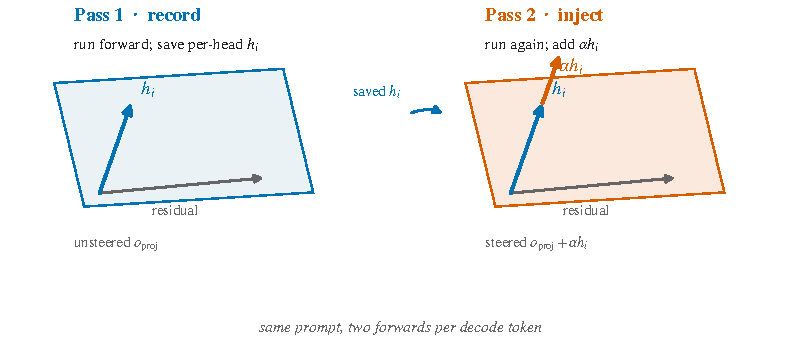
\includegraphics[width=0.55\linewidth]{figures/fig1_juice_dualrun.pdf}
\caption{Dual-run JuICE. Pass 1 records $h_i$ after \texttt{o\_proj}; pass 2 injects $\alpha h_i$.}
\label{fig:juice-dualrun}
\end{figure}
Pass 1 records per-head outputs after \texttt{o\_proj}; pass 2 adds $\alpha$ times the saved vector. Context uses $K{=}10$ (and $K{=}5$); parametric uses clean/noisy $K{=}2$ and $K{=}3$; Gemma also uses $K{=}1$ on the raw peak. Default transfer is enlarge-only, $\alpha{+}{=}1$, $\alpha{-}{=}0$. Suppression cells use $\alpha{+}{=}0$, $\alpha{-}{=}1$. Eval is \texttt{juice\_coherent}, greedy, $\texttt{max\_new\_tokens}{=}16$. Labels are $\{\texttt{parametric}, \texttt{context}, \texttt{rejects\_context}, \texttt{other}\}$; $\texttt{follows\_context}$ is $\texttt{label}{==}\texttt{``context''}$. A letter heuristic stayed at 100\% while $\alpha{=}3/5$ \texttt{other} hit 50--64\%, so we report label counts. Scorer brevity/parametric-first behavior is documented in Appendix~\ref{app:reverse}.

Paired bootstrap, 1000 draws, seed 42, percentile 95\% CI, throughout. Stage~1 resamples 164 items. Stage~2 $\Delta$ is steered minus baseline \texttt{follows\_context} on the 50 eval IDs. ``Excludes 0'' is the detection rule. CIs are whole percentage points. Random-$K$ excludes the FP16 identified set. Gemma suppress specificity is $\Delta_{\mathrm{id}}-\Delta_{\mathrm{random}}$; DiD is $\mathrm{spec}_{INT4}-\mathrm{spec}_{FP16}$. We do not infer specificity from overlapping cell CIs.

The pre-registered Llama gate required same-sign transfer of context K10/K5 and parametric clean K2 at coherence $\ge 0.90$; magnitude match was not required. That gate passed. After CIs, repairs, and reverse-transfer diagnostics we report a narrower sentence: context K10 is the detected INT4 effect in forward transfer and native apply, not in reverse transfer; parametric steering is a null at $\alpha{=}1$ plus failed repairs. On Gemma the Llama objects do not map one-to-one: we report L27\_H6 $K{=}1$ as the detected transferable object (random-$K{=}1$ is a hard zero), directional context K10 enlarge and directional parametric K2 as FP16 nulls, and context suppress as a detected effect whose identified-versus-random contrast is not. Native INT4 re-ID and reverse transfer were not run on Gemma.

\section{Results}
\label{sec:results}

\subsection{Stage 1: behavioral arbitration on Instruct}
\label{sec:stage1}

Stage~1 asks, before any head is identified: when a fact survives INT4, does conflict arbitration still look like FP16? We compare FP16 Instruct to a third-party GPTQ-INT4 Instruct checkpoint on 250 ConflictQA popular items, then restrict to the 164 items closed-book correct at both precisions.

\begin{table}[t]
\caption{Stage~1 memorization rate. MR$^\star$ is the primary behavioral estimand (shared 164).}
\label{tab:mrstar}
\centering
\small
\begin{tabular}{lccc}
\toprule
Precision & Closed-book & MR (unfiltered) & MR$^\star$ (shared 164) \\
\midrule
FP16 & 182/250 (72.8\%) & 92/250 (36.8\%) & \textbf{76/164 (46.3\%)} \\
INT4 & 175/250 (70.0\%) & 48/250 (19.2\%) & \textbf{37/164 (22.6\%)} \\
\bottomrule
\end{tabular}
\end{table}

MR$^\star$ on the shared 164 is the primary estimand (Table~\ref{tab:mrstar}): INT4 $-23.8$~pp $[-31.7,-17.1]$, excluding 0. Closed-book is nearly stable ($-7$ items); unfiltered MR also drops $-17.6$~pp, so this is not forgetting that vanishes after the double filter. Cluster-robust logit AME on \texttt{follows\_context} is $+10.3$~pp $[+3.1,+17.5]$ (Table~\ref{tab:ame}). Label counts (Appendix Tables~\ref{tab:labels}--\ref{tab:transitions}) show a parametric collapse and a rise in context. A first-pass substring scorer inflated AME ($+20.6$~pp) by counting denials as context; numbers here use the corrected scorer. Llama-3.2-1B-Instruct was a null screen and is not mixed into the 8B claim. Stage~1 and Stage~2 INT4 files remain different artifacts.

\begin{table}[t]
\caption{Stage~1 \texttt{follows\_context} AME on the shared 164 items. The cluster-robust logit row is the published estimand.}
\label{tab:ame}
\centering
\small
\begin{tabular}{lccc}
\toprule
Estimand & Point & 95\% CI & excl.\ 0? \\
\midrule
Cluster-robust logit AME & $\mathbf{+10.3}$~\textbf{pp} & $\mathbf{[+3.1, +17.5]}$ & yes \\
Raw $\Delta P(\texttt{context})$ & $+10.4$~pp & $(52{\to}69)/164$ & --- \\
Item-averaged AME & $+9.8$~pp & --- & --- \\
Mixed VB AME & $+16.1$~pp & $[+5.9, +26.2]$ & yes \\
\bottomrule
\end{tabular}
\end{table}

\subsection{Instruct is the wrong mechanistic target}
\label{sec:instruct-base}

JuICE was developed on base models \citep{li2025taming}. On Instruct with a chat template, parametric ID and steering fail (Table~\ref{tab:instruct-base}): directional\_par is suppressed $\sim$1100$\times$. That is a model+prompt confound. All INT4 transfer cells use base-identified heads.

\begin{table}[t]
\caption{Instruct (chat template) vs.\ base (plain JuICE prompts). Parametric directional ID is suppressed on Instruct.}
\label{tab:instruct-base}
\centering
\footnotesize
\setlength{\tabcolsep}{3pt}
\begin{tabular}{p{2.05in}cc}
\toprule
 & Instruct (chat) & Base (plain JuICE prompts) \\
\midrule
Raw enlarge Jaccard (ctx vs par H+) & $\mathbf{0.54}$ & $\mathbf{0.053}$ \\
Peak raw \texttt{scores\_pos} (ctx / par) & $0.0080$ / $0.0077$ & $\mathbf{0.036}$ / $\mathbf{0.058}$ \\
Best \texttt{directional\_par} & $\mathbf{2.68\times 10^{-4}}$ & $\mathbf{0.304}$ ($\sim$1130$\times$) \\
Directional top-10 Jaccard (ctx vs par) & $0$ & $0$ \\
Parametric Cell-3 at $\alpha{+}{=}1$ & $0$ / $-2$~pp ($K{=}2$ / $K{=}3$) & $\mathbf{-6}$ to $\mathbf{-8}$~pp \\
Context Cell-3 at $\alpha{+}{=}1$ & $+6$ to $+8$~pp & $+6$ to $+10$~pp \\
\bottomrule
\end{tabular}
\end{table}

FP16 base must steer before transfer. Table~\ref{tab:fp16-gate}: context K10 $+10$ $[+2,+20]$; clean K2 (L20\_H14, L26\_H15) $-8$ $[-16,-2]$. Those locked heads are applied to INT4 without re-ID.

\begin{table}[t]
\caption{FP16 base steering on the 50 eval items. The letter-heuristic column is 100\% in every row.}
\label{tab:fp16-gate}
\centering
\footnotesize
\setlength{\tabcolsep}{3pt}
\begin{tabular}{lccccc}
\toprule
Condition & Heads & $fc$ & $\Delta$ & Coh & P/C/O \\
\midrule
baseline & --- & 16\% & --- & 100\% & 40/8/2 \\
context K10 & directional ctx top-10 & 26\% & $\mathbf{+10}$ & 100\% & 34/13/3 \\
context K5 & top-5 of those & 22\% & $+6$ & 100\% & 36/11/3 \\
parametric K2 & L20\_H14, L31\_H14 & 10\% & $-6$ & 100\% & 39/5/6 \\
parametric K3 & + L26\_H15 & 10\% & $-6$ & 100\% & 39/5/6 \\
parametric clean K2 & \textbf{L20\_H14, L26\_H15} & 8\% & $\mathbf{-8}$ & 100\% & 42/4/4 \\
\bottomrule
\end{tabular}
\end{table}

\subsection{Context K10 transfers, and is head-specific}
\label{sec:ctx-transfer}

FP16 context K10, applied unchanged to canonical INT4 ($\mathrm{N_{CALIB}{=}128}$), raises \texttt{follows\_context} by $+18$ $[+8,+30]$ (Table~\ref{tab:ctx-k10}, Figure~\ref{fig:deltas}). A random-K10 control is $-6$ $[-14,0]$ (includes 0): identified excludes 0, random does not. CIs overlap at $n{=}50$, so this is control-fails / treatment-detects, not a proven difference of deltas. Context K5 was not re-run at $N{=}128$; at $N{=}64$ it was $+6$ $[-2,+16]$. Re-quantizing at $N{=}64$ vs.\ $128$ flips no excludes-0 call (Figure~\ref{fig:n64-n128}; Table~\ref{tab:n64-n128}). The same-sign gate passed; after CIs the only detected INT4 effect is context K10.

\begin{figure}[t]
\centering
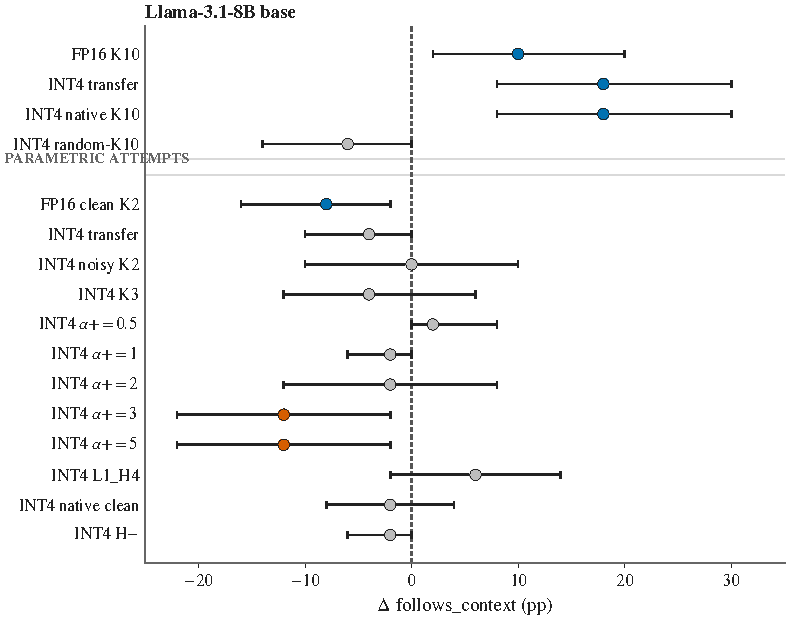
\includegraphics[width=\linewidth]{figures/fig2_delta_follows_context.pdf}
\caption{$\Delta$ \texttt{follows\_context} on 50 items (1000 paired draws, seed 42). Teal: CI excludes 0; grey: includes 0; hatch: $\alpha{=}3/5$ \texttt{other}-inflation.}
\label{fig:deltas}
\end{figure}

\begin{table}[t]
\caption{Forward transfer of FP16 context K10 onto canonical INT4 ($\mathrm{N_{CALIB}{=}128}$).}
\label{tab:ctx-k10}
\centering
\footnotesize
\setlength{\tabcolsep}{2.5pt}
\begin{tabular}{lcccccc}
\toprule
Condition & INT4 $fc$ & INT4 $\Delta$ [95\% CI] & excl.\ 0? & FP16 $\Delta$ [CI] & Sign vs FP16 & P/C/O \\
\midrule
baseline & 20\% & --- & --- & 16\% & --- & 39/10/1 \\
\textbf{context K10} & 38\% & $\mathbf{+18}$ $\mathbf{[+8, +30]}$ & \textbf{yes} (1000/1000 +) & $+10$ $[+2, +20]$ & same & 28/19/3 \\
\bottomrule
\end{tabular}
\end{table}

\begin{figure}[t]
\centering
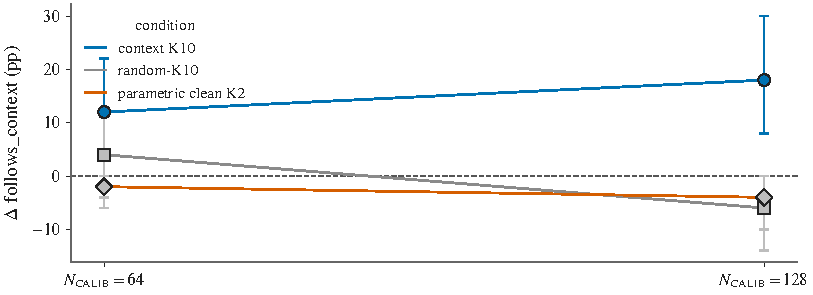
\includegraphics[width=\linewidth]{figures/fig4_n64_vs_n128.pdf}
\caption{GPTQ $N_{\mathrm{CALIB}}$ robustness. Filled: CI excludes 0. No detection call flips.}
\label{fig:n64-n128}
\end{figure}

\subsection{Reverse transfer and native in-precision identification}
\label{sec:reverse}

Native INT4 context K10 applied in-precision (Cell~B) reproduces the forward-transfer $+18$ $[+8,+30]$; reverse transfer of those heads onto FP16 (Cell~A) is a large scorer-level positive that we reject as the same circuit. Manual-inspection counts, head-level ID sign flips, and the $\alpha$-sweep (exam-meta 36--58\%) are in Appendix~\ref{app:reverse}. We do not claim bidirectional transfer.

\subsection{Parametric direction: a complete negative}
\label{sec:parametric}

FP16 clean K2 is a detected $-8$ $[-16,-2]$. On INT4 every repair we ran is a null or a collapse at $\alpha{=}1$ (Figure~\ref{fig:deltas}b); full counts are Appendix~\ref{app:parametric}. (0)~Transfer of L20\_H14+L26\_H15 is $-4$ $[-10,0]$ at $N{=}128$ and $-2$ $[-6,0]$ at $N{=}64$, both including 0. (1)~Rescale $\alpha{+}{\in}\{0.5,1,2,3,5\}$ never restores the FP16 object; $\alpha{=}3/5$ ``detections'' are 50--64\% \texttt{other}. (2)~Steering the raw peak L1\_H4 is $+6$ $[-2,+14]$, wrong sign. (3)~Native directional top-2 is the same noisy pair (Jaccard 1.0) and does not steer; native clean L16\_H30/L17\_H27 is $-2$ $[-8,+4]$. (4)~Context H$-$ is $-2$ $[-6,0]$. FP16-vs-INT4 Jaccard sits inside the $|\mathcal{D}|{=}4$ noise floor. This is a thorough negative, not weaker-but-real attenuation.

\subsection{Directional re-ranking has a blind spot}
\label{sec:blindspot}

The parametric repairs above used directional ranking, $\texttt{directional\_par} := \texttt{par\_pos} - \texttt{ctx\_pos}$.
\begin{wrapfigure}{r}{0.45\textwidth}
\centering
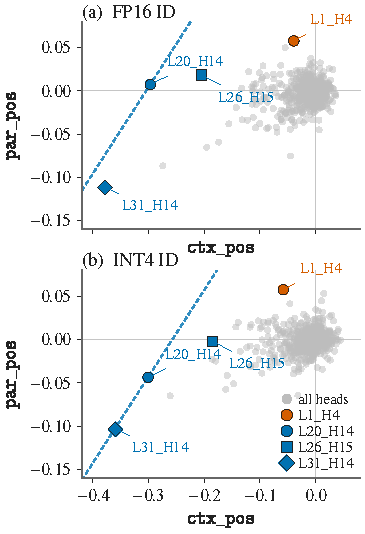
\includegraphics[width=\linewidth]{figures/fig3_directional_blindspot.pdf}
\caption{Per-head \texttt{ctx\_pos} vs.\ \texttt{par\_pos}. Dashed line: constant \texttt{directional\_par} through L20\_H14. L20\_H14 and L31\_H14 rank by context suppression; L1\_H4 is the raw \texttt{par\_pos} peak (\#29 / \#14).}
\label{fig:blindspot}
\end{wrapfigure}
\begin{flushleft}
That score can promote heads that suppress context tokens a lot, via a large negative $\texttt{ctx\_pos}$, over heads that actually boost parametric tokens (Figure~\ref{fig:blindspot}, Table~\ref{tab:blindspot}). The INT4 noise proxy, median $\max(|\texttt{ctx}|,|\texttt{par}|)$, is $9.2\times 10^{-3}$, so the $5\times$ threshold is $0.046$. Only L1\_H4 in or near the top 20 clears that threshold with positive $\texttt{par\_pos}$. Directional top-$K$ is therefore not interchangeable with the raw parametric peak without checking the sign of \texttt{par\_pos}.
\end{flushleft}

\begin{table}[t]
\caption{Directional re-ranking vs.\ raw parametric enlarge. L1\_H4 is the raw peak on both precisions and is ranked \#29 / \#14 by \texttt{dir\_par}.}
\label{tab:blindspot}
\centering
\footnotesize
\setlength{\tabcolsep}{2.5pt}
\begin{tabular}{p{0.55in}p{1.15in}p{1.7in}p{1.7in}}
\toprule
Head & Role & FP16 $\texttt{par\_pos}$ / $\texttt{ctx\_pos}$ / \texttt{dir\_par} (rank) & INT4 $\texttt{par\_pos}$ / $\texttt{ctx\_pos}$ / \texttt{dir\_par} (rank) \\
\midrule
\textbf{L1\_H4} & raw parametric enlarge \textbf{\#1} on both precisions & $\mathbf{+0.0577}$ / $-0.0392$ / $+0.0969$ (\textbf{\#29}) & $\mathbf{+0.0578}$ / $-0.0581$ / $+0.1159$ (\textbf{\#14}) \\
L20\_H14 & directional \#1; in clean + noisy K2 & $+0.0072$ / $-0.297$ / $\mathbf{+0.304}$ (\textbf{\#1}) & $\mathbf{-0.0436}$ / $-0.301$ / $+0.257$ (\textbf{\#1}) \\
L31\_H14 & noisy K2 (ctx-suppression) & $-0.112$ / $-0.378$ / $+0.267$ (\#2) & $-0.104$ / $-0.360$ / $+0.256$ (\#2) \\
L26\_H15 & clean K2 & $+0.0184$ / $-0.205$ / $+0.223$ (\#3) & $-0.0019$ / $-0.185$ / $+0.183$ (\#4) \\
\bottomrule
\end{tabular}
\end{table}

\subsection{Gemma-2-9B: the transferable object is the raw parametric peak}
\label{sec:model2}

We repeat identify$\times$apply on Gemma-2-9B \citep{team2024gemma2} with the same 50 items and GPTQ recipe. Native INT4 re-ID and reverse transfer were not run. Figure~\ref{fig:cross-family}: Llama transfers context K10; Gemma transfers one raw parametric head.

\begin{figure}[t]
\centering
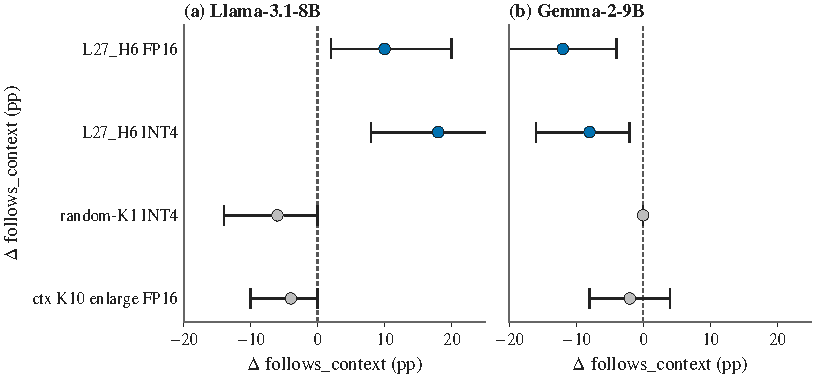
\includegraphics[width=\linewidth]{figures/fig6_cross_family.pdf}
\caption{Which object transfers, by family. Teal: CI excludes 0; grey: includes 0. Same 50 items, 1000 paired draws, seed 42.}
\label{fig:cross-family}
\end{figure}

Directional ctx vs par top-10 Jaccard is $0.0$. Clean par K2 (L31\_H7, L39\_H6) are context suppressors; the raw peak is L27\_H6 ($\texttt{par\_pos}{=}+0.027$; Figure~\ref{fig:gemma-blindspot}). FP16 baseline is 48\%. Table~\ref{tab:gemma-fp16}: ctx K10 enlarge $-2$ $[-8,+4]$; par K2 $-2$ $[-8,+4]$; \textbf{L27\_H6 $-12$ $[-22,-4]$}. INT4 transfer of L27\_H6 is $-8$ $[-16,-2]$ vs random-$K{=}1$ exactly $0$. Context suppress of the directional K10 is $-12$ $[-24,-2]$ on FP16 and $-8$ $[-16,-2]$ on INT4, but INT4 random H$-$ is also $-12$ $[-24,-2]$. Paired specificity FP16 $-6$ $[-18,+6]$, INT4 $+4$ $[-8,+16]$, DiD $+10$ $[-4,+24]$---all include 0 (Table~\ref{tab:gemma-suppress-did}, Figure~\ref{fig:gemma-deltas}b). Step-by-step ID lists, flips, and the cell-CI vs DiD argument: Appendix~\ref{app:gemma}.

\begin{wrapfigure}{r}{0.45\textwidth}
\centering
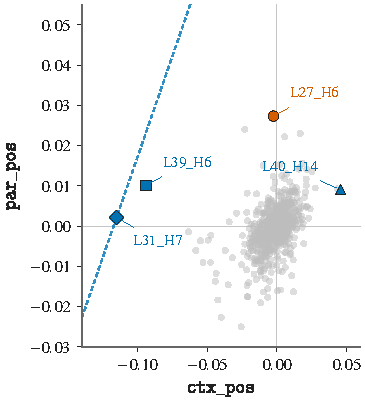
\includegraphics[width=\linewidth]{figures/fig7_gemma_blindspot.pdf}
\caption{Gemma FP16 ID. L27\_H6 is the raw $\texttt{par\_pos}$ peak; L31\_H7/L39\_H6 rank by suppression.}
\label{fig:gemma-blindspot}
\end{wrapfigure}

\begin{table}[t]
\caption{Gemma-2-9B Cell-3 (FP16) and L27\_H6 forward transfer (INT4 $\mathrm{N_{CALIB}{=}128}$). Letter heuristic 100\%. INT4 baseline 46\% (23/23/4).}
\label{tab:gemma-fp16}
\label{tab:gemma-l27}
\centering
\footnotesize
\setlength{\tabcolsep}{3pt}
\begin{tabular}{lcccc}
\toprule
Condition & Heads / notes & $fc$ or $\Delta$ [95\% CI] & excl.\ 0? & P/C/O \\
\midrule
FP16 baseline & --- & 48\% & --- & 22/24/4 \\
FP16 ctx K10 enlarge & directional top-10 & $-2$ $[-8,+4]$ & no & 23/23/4 \\
FP16 par K2 clean & L31\_H7, L39\_H6 & $-2$ $[-8,+4]$ & no & 23/23/4 \\
\textbf{FP16 par K1 raw} & \textbf{L27\_H6} & $\mathbf{-12}$ $\mathbf{[-22,-4]}$ & \textbf{yes} & 28/18/4 \\
FP16 random-K10 enlarge & seed 42, exclude ID union & $-6$ $[-14,+2]$ & no & 27/21/2 \\
\midrule
\textbf{INT4 L27\_H6 $K{=}1$} & same locked head & $\mathbf{-8}$ $\mathbf{[-16,-2]}$ & \textbf{yes} & 27/19/4 \\
INT4 random $K{=}1$ & L40\_H15 & $0$ $[0,0]$ & no & 23/23/4 \\
\bottomrule
\end{tabular}
\end{table}

\begin{figure}[t]
\centering
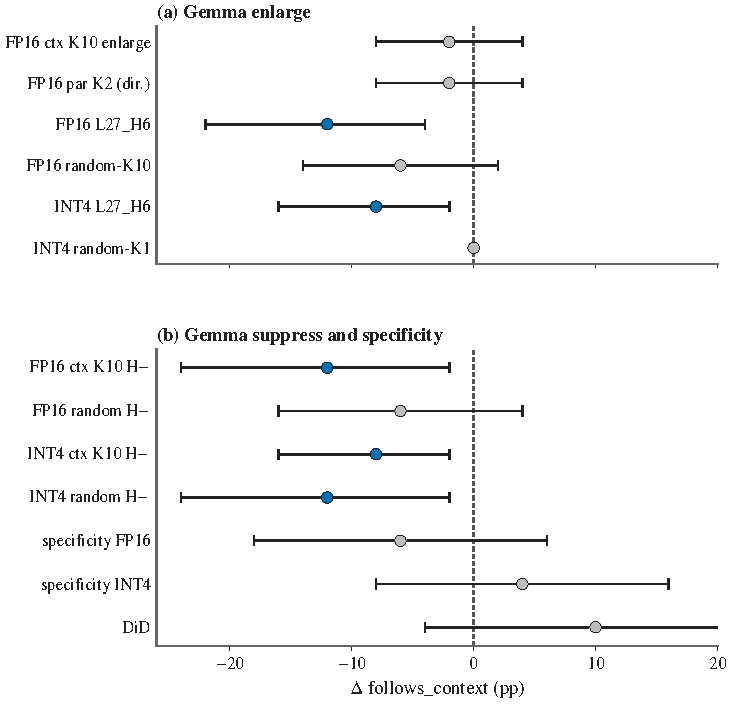
\includegraphics[width=\linewidth]{figures/fig5_gemma_deltas.pdf}
\caption{Gemma $\Delta$ \texttt{follows\_context}. (a)~Only L27\_H6 is a detected enlarge. (b)~Suppress is detected for identified and INT4 random; specificity and DiD include 0.}
\label{fig:gemma-deltas}
\end{figure}

\section{Discussion}
\label{sec:discussion}

The two families reject a category-level account of transfer (Figure~\ref{fig:cross-family}). Llama's head-specific forward transfer is context-directed; Gemma's is the raw parametric peak L27\_H6. Conversely, Llama's FP16 parametric steer is not detected on INT4 despite rescaling, raw-peak, and native re-identification attempts, while Gemma's directional context K10 enlarge is already a FP16 null. The evidence supports neither ``context survives compression'' nor ``parametric memory breaks.'' Rather, whether a particular causal object transfers is model- and direction-dependent under this GPTQ recipe.

The cross-family regularity is methodological. In both families, the directional score $\texttt{par\_pos}-\texttt{ctx\_pos}$ elevates context suppressors above the strongest positive parametric signal. On Llama, checking the raw peak did not recover a useful INT4 parametric steer; on Gemma, checking it discovered the only detected FP16-to-INT4 parametric transfer. Directional top-$K$ should therefore not be treated as interchangeable with a source-specific circuit without inspecting the underlying positive score and applying an intervention.

Our controls also separate an intervention effect from a circuit claim. Llama context K10 passes a random-head control in forward transfer and is reproduced by native INT4 identification and application; the reverse INT4-to-FP16 result is rejected after text inspection reveals an exam-meta artifact. Gemma context suppression moves behavior at both precisions, but its identified-versus-random contrast is not detected. Reporting only the identified cell would have overstated the result. More generally, a same-sign output effect does not establish that the identified causal object, rather than a generic intervention of the same size, survived compression.

% The former prospective second-model checklist was removed after completing Gemma-2.

\section{Conclusion}
\label{sec:conclusion}

If a source-arbitration intervention is computed in FP16 residual-stream geometry, GPTQ INT4 does not apply a uniform tax to that object. On Llama-3.1-8B base, context K10 survives compression in the forward direction and in-precision, head-specifically; parametric JuICE does not, at this $n$, after the repairs we ran. On Gemma-2-9B base the category pattern reverses: a single raw parametric head transfers head-specifically, and context enlarge does not. In both families, directional ranking promotes context suppressors over the strongest positive parametric signal, and a detected output effect is not the same as a detected identified-versus-random contrast. Circuit-level claims about quantization therefore require the identify$\times$apply design, a random-head control, and a look at the completions---not a source label and a same-sign $\Delta$.

\section{Limitations}
\label{sec:limitations}

Every caveat flagged in the locked findings is load-bearing.

The parametric null is a detection failure at this $n$, not a proof that the FP16 object is absent. Stage~2 evaluation uses 50 held-out items on a 2~pp grid. The parametric clean-K2 transfer CI $[-10, 0]$ on the canonical checkpoint includes 0 and is compatible with a true delta of 0; it is also compatible with a small negative that this $n$ cannot detect. Head identification is similarly thin.

Head-set drift is not identifiable at this calibration size except as the observation that top-2 parametric is stable. Identification used four calibration items. Observed FP16-versus-INT4 overlap sits within the INT4-versus-INT4 noise floor for every spec we computed. Jaccard noise uses 25 draws. The quantization recipe is equally specific.

All INT4 results are GPTQ at 4-bit with group size 128. We did not test AWQ, bitsandbytes, or other recipes. Claims are about this GPTQ INT4 object, not about quantization in general. Even within that recipe, the unsteered baseline is not perfectly stable.

Unsteered INT4 \texttt{follows\_context} shifted from 14\% to 20\% between the $N{=}64$ and $N{=}128$ checkpoints on the same 50 eval ids. Steered deltas are paired against their own session's baseline and did not change detection calls, so this does not undermine the $\Delta$ results. It does mean that the baseline rate itself shows some calibration sensitivity. The two stages also do not share a weight file.

Stage~1 and Stage~2 use different INT4 artifacts. Stage~1 is a third-party Instruct GPTQ; Stage~2 is a self-quantized base checkpoint, with headline $\mathrm{N_{CALIB}{=}128}$ and $N{=}64$ retained only for comparison. Recovery arms (the $\alpha$-grid, L1\_H4, native directional K2/K3, and H$-$) were run on $N{=}64$ and were not repeated at $N{=}128$; native apply of the clean pair was run at $N{=}128$. Scoring choices further bound what those cells can say.

AME still uses equality to \texttt{``context''} only; breakdowns keep \texttt{rejects\_context}. The letter heuristic stayed at 100\% while $\alpha{=}3/5$ \texttt{other} hit 50--64\%, which is why we report label counts rather than the heuristic alone. The parametric-first / brevity pattern is a pipeline property of the scorer on \texttt{juice\_coherent} completions. Cluster-robust AME $+10.3$ $[+3.1, +17.5]$ is from the Stage~1 memo, not a re-fit in this writeup. The 1B null/confound screen is not mixed into the 8B claim. Instruct Cell-3 parametric $0/-2$~pp has no paired bootstrap.

The empirical scope is two base-model families, one GPTQ recipe, and conflict items from ConflictQA popular. Stage~2 still has only 50 evaluation items and four head-identification calibration items per family. Gemma Stage~2 is base only: there is no Gemma Instruct MR$^\star$, no native INT4 re-identification, and no reverse transfer; those cells are not filled from Llama. The Gemma context-suppression identified-minus-random contrasts and their difference-in-differences all include zero; they are reported as inconclusive rather than as evidence of circuit specificity or specificity loss. Gemma's unsteered INT4 baseline was 46\% against FP16 48\% on the same 50 items. This is not a claim about all LLMs, production RAG, or bidirectional circuit transfer.

\subsection*{Reproducibility statement}

(This section is recommended and does not count toward the page limit.)

Paired bootstrap is the detection protocol throughout. Stage~1 resamples the 164 double-filtered items; Stage~2 resamples the 50 eval items. Both use 1000 draws and a percentile 95\% CI, with seed 42 throughout (random-$K$ additionally uses seeds 42--45). Decode is greedy at $T{=}0$. Head-identification calibration IDs, the eval split, locked head sets, and the GPTQ recipe ($\mathrm{N_{CALIB}}$, group size, \texttt{sym}, \texttt{desc\_act}) are specified in \S\ref{sec:methods}. Code and data will be released in anonymized form with the submission as anonymous supplementary material. This statement does not itself contain the reproduction recipe; the recipe is \S\ref{sec:methods}--\S\ref{sec:results}.

\subsection*{AI use disclosure}
\label{sec:ai}

(This section is \textbf{required} and does not count toward the page limit.)

We used generative AI tools to assist with code implementation, debugging, figure ideation, and language editing. The authors designed the experiments, ran and inspected all analyses, verified reported numbers against saved outputs, and take responsibility for the manuscript's methods, claims, and conclusions.

\clearpage
\appendix

\section{Reverse transfer and native identification}
\label{app:reverse}

Forward transfer shows that FP16's context K10 still works on INT4. That does not yet say whether INT4 has its own context circuit, or whether that circuit is the same object when applied back on FP16. We add two cells on the same 50 items, $\alpha{+}{=}1$, $\alpha{-}{=}0$ unless noted, and the same paired bootstrap (1000 draws, seed 42). Cell~A is reverse transfer: identify a directional context K10 on INT4 and apply those heads on FP16. Cell~B is native identification: apply that same INT4 K10 back on the $\mathrm{N_{CALIB}{=}128}$ INT4 checkpoint. The native INT4 set is L7\_H26, L14\_H10, L7\_H21, L4\_H5, L3\_H3, L31\_H20, L4\_H11, L14\_H23, L8\_H29, L9\_H0. Jaccard versus FP16 K10 is $0.33$ (overlap 5/15: L7\_H26, L4\_H5, L31\_H20, L14\_H23, L9\_H0). Baselines are reused from prior sessions.

\begin{table}[h]
\caption{Identify$\times$apply triangulation for context K10. Cell~B is confirmed as a native in-precision effect; Cell~A is rejected as a scorer artifact rather than the same circuit running in reverse.}
\label{tab:cells}
\centering
\footnotesize
\setlength{\tabcolsep}{2pt}
\begin{tabular}{lp{1.15in}ccp{1.7in}}
\toprule
Cell & Identify $\to$ apply & $fc$ & $\Delta$ [95\% CI] & Comparator \\
\midrule
\textbf{A reverse} & INT4 K10 $\to$ FP16 & 64\% & $\mathbf{+48}$ $\mathbf{[+34, +62]}$ yes (1000/1000 +) & FP16-ID K10 on FP16: $\mathbf{+10}$ $\mathbf{[+2, +20]}$ \\
\textbf{B native} & INT4 K10 $\to$ INT4 $N128$ & 38\% & $\mathbf{+18}$ $\mathbf{[+8, +30]}$ yes (1000/1000 +) & FP16-ID K10 on INT4 $N128$: $\mathbf{+18}$ $\mathbf{[+8, +30]}$ \\
\bottomrule
\end{tabular}
\end{table}

Letter-heuristic coherence remained at 100\% in both cells. Cell~B reproduces the forward-transfer magnitude on both native INT4 apply and FP16-heads-on-INT4. Manual inspection rules out a Cell~A-style scorer trap: exam-meta is $0/19$ among context labels and $0/50$ under any label; $16/19$ context ids match forward transfer; $11/19$ texts are identical; $40/50$ items keep the same label. The 7 \texttt{other} labels are alias or brevity misses (\texttt{Lahore} versus gold ``The Indomitable City''; bare \texttt{Kangra} / \texttt{Osona} / \texttt{Yungay Province}), not format collapse. Completions are on-topic context-entity names in the same style as the trusted FP16-to-INT4 run. FP16's own K10, FP16 heads transferred onto INT4, and INT4's own K10 applied in-precision therefore all move \texttt{follows\_context} the same way, and two of those three cells have been read as text.

Cell~A is a rejected same-circuit hypothesis, not a silent drop. The scorer records a real, $\alpha$-driven positive at $\alpha{=}1$ whose CI excludes 0 (Table~\ref{tab:cells}). Manual inspection shows a different behavioral object than FP16's own K10 or the forward-transfer result: $13/32$ context labels at $\alpha{=}1$ are bare context-entity names followed by exam-meta (``Edina / Rumbek / \ldots Note: The question is a multiple-choice question\ldots''). Letter-heuristic coherence stays at 100\%. The failure is in cross-precision application, not in INT4 identification quality. On INT4's own ID, 9/10 of the native K10 heads are context-specific ($\texttt{ctx\_pos}{>}0$ and $\texttt{par\_pos}{\le}0$); L8\_H29 is the exception ($\texttt{par\_pos}$ $+0.0009$). That is not a universal-booster ID signature---FP16's own K10 is $0/10$ both-positive on FP16 ID. Two INT4-only heads are context-negative when scored on FP16 ID: L7\_H21 has $\texttt{ctx\_pos}$ $-0.0058$ (INT4 ID $+0.0120$) and L3\_H3 has $\texttt{ctx\_pos}$ $-0.0185$ (INT4 ID $+0.0217$). Steering that set on FP16 is not the same K10.

The FP16 $\alpha$-sweep with the same heads and reused baseline is Table~\ref{tab:cell-a-alpha}. A scaled copy of FP16's own K10 ($+10$ $[+2, +20]$) should have dropped toward about $+10$ at $\alpha{=}0.25$ and $0.5$ and lost the exam-meta dump. It did not. The floor remains a large positive ($+34$ at $\alpha{=}0.25$), with more exam-meta at low $\alpha$ (58\%), not less. The \texttt{other} count stays in the single digits, unlike the $\alpha{=}3/5$ parametric collapse. $\Delta$ still rises with $\alpha$, so something is being driven: format and scorer collapse, not genuine context-arbitration. We are not claiming symmetric bidirectional transfer. Context-following steering is robust within each precision---FP16 own K10, INT4 native K10, and FP16-to-INT4 forward transfer---and does not reverse-transfer cleanly.

The scorer has a pipeline property that matters for both Cell~B and the trusted forward-transfer cell. Some parametric-to-context flips occur when the unsteered INT4 baseline already named the context entity in a full sentence, labeled \texttt{parametric} because the matcher checks parametric gold first, and steering shortens the completion to a bare name that then labels \texttt{context}. All 9 such flips in the native INT4 cell are of this kind. The pattern is a property of the scorer on \texttt{juice\_coherent} completions wherever context-K10 shortening occurs, not a cell-specific artifact. We therefore report label counts and read a sample of texts.

\section{Parametric recovery attempts: full detail}
\label{app:parametric}

On FP16, the clean K2 pair is a real effect of $-8$~pp whose CI excludes 0. On INT4, every path we tested fails to recover a usable parametric steer. Recovery arms---the $\alpha$-grid, L1\_H4, native directional K2/K3, and context H$-$---were run on the $N{=}64$ checkpoint and were not repeated at $N{=}128$. The native clean pair is the exception: it was identified on $N{=}64$ and applied on $N{=}128$.

\paragraph{0. Transfer of the FP16 clean pair.}
The starting test applies L20\_H14 and L26\_H15 at $\alpha{+}{=}1$, $\alpha{-}{=}0$. On the canonical $\mathrm{N_{CALIB}{=}128}$ checkpoint the delta is $-4$~pp $[-10, 0]$, which includes 0. Of 1000 bootstrap draws, 858 are negative, 142 are zero, and 0 are positive. Coherence remained at 100\%, with P/C/O 37/8/5. The interval is compatible with a true delta of 0. It is not a sign flip, not a collapse, and not a detected effect. The $\mathrm{N_{CALIB}{=}64}$ check on the same locked pair and same 50 items is $-2$~pp $[-6, 0]$, which also includes 0 (622/1000 negative, 378 zero, 0 positive; coherence 100\%; P/C/O 41/6/3). The parametric null is therefore not an artifact of $\mathrm{N_{CALIB}{=}64}$. Related transfer arms on the $N{=}64$ cell, not re-run at $N{=}128$, are noisy K2 L20\_H14+L31\_H14 at $0$ $[-10, +10]$ (a sign flip versus FP16 $-6$) and K3 at $-4$ $[-12, +6]$, which includes 0.

\paragraph{1. Alpha grid on the same clean pair.}
If INT4 merely rescaled the same axis, a different $\alpha{+}$ should restore the FP16 $-8$~pp object. Table~\ref{tab:alpha-grid} reports $\alpha{+} \in \{0.5, 1, 2, 3, 5\}$ with $\alpha{-}{=}0$ and $n{=}50$. The letter heuristic remains at 100\% at every gain. At $\alpha{=}3$ and $5$, however, \texttt{other} is 50--64\%: fluent-looking rambling, blank-slot, and off-entity completions, not parametric answers. Context does not convert to parametric. The $-12$~pp detections at $\alpha{=}3/5$ are therefore not recovered parametric steering. Rescale does not restore the FP16 object.

\paragraph{2. L1\_H4, the raw parametric peak.}
A different-head repair asks whether INT4's raw parametric peak, rather than the directional pair, is the missing object. L1\_H4 is the only INT4 (and FP16) head with $\texttt{par\_pos}$ above $5\times$ the identification noise floor. Steering $K{=}1$ at $\alpha{+}{=}1$, $\alpha{-}{=}0$ yields $+6$ $[-2, +14]$, which includes 0, and has the wrong sign for a parametric enlarge: more context-following, not less. Of 1000 draws, 882 are positive. Coherence remained at 100\%, with P/C/O 36/10/4. The story that one should simply steer the same raw peak is rejected.

\paragraph{3. Native INT4 re-identification.}
If the FP16 pair was the wrong pair, native re-identification should return a different one that steers. We used the same protocol as FP16 base: $|\mathcal{D}|{=}4$ (the same four calibration IDs), three-type JuICE prompts, and FAST alphas (Table~\ref{tab:native-id}). Native directional top-2 is not a different pair; it is FP16's noisy K2, which does not steer on INT4. The native clean filter, $\texttt{par\_pos}{>}0$ and $\texttt{dir\_par}{>}0$, does return a different pair, L16\_H30 and L17\_H27. Applied on the $\mathrm{N_{CALIB}{=}128}$ checkpoint at $K{=}2$, $\alpha{+}{=}1$, $\alpha{-}{=}0$, same 50 items, seed 42, that pair yields $-2$~pp $[-8, +4]$, which includes 0 (622/1000 negative, 214 zero, 164 positive). Coherence remained at 100\%. Parametric count is unchanged at 39; context $10{\to}9$, other $1{\to}2$. The in-session baseline matched the $N{=}128$ transfer session item-for-item (\texttt{identical: true}, $fc$ 20\%). No FP16 same-sign gate applies, because Jaccard versus L20\_H14/L26\_H15 is $0.00$. This is a null, not a repair: near-noise $\texttt{par\_pos}$ ($+0.020$ / $+0.015$) did not become a usable parametric steer. Random parametric K2 moves the wrong way ($+4$ $[0, +10]$).

\paragraph{4. Context-suppression as a parametric proxy.}
A last repair treats context suppression as a parametric proxy: H$-$ is the FP16 directional context K10, enlarge empty, $\alpha{+}{=}0$, $\alpha{-}{=}1$. The delta is $-2$ $[-6, 0]$, which includes 0, with P/C/O 44/6/0. That is the same one-item nudge as clean K2 at $\alpha{=}1$.

\paragraph{Jaccard vs.\ $|\mathcal{D}|{=}4$ noise.}
Head-set overlap is not identifiable at this calibration size. Twenty-five calibration-item resamples place every observed FP16-versus-INT4 Jaccard we computed within the INT4-versus-INT4 noise floor (context K10 $J{=}0.33$ versus noise mean $0.27$ $[0.05, 0.82]$; parametric K2 $J{=}1.0$ versus noise already about $0.95$). The exception, such as it is, is that top-2 parametric is stable. The Jaccard noise uses 25 draws.

Taken together, this is a thorough negative, not a weaker-but-real attenuation. It is not a clean rescale story, because rescale failed without producing parametric answers. It is not a clean ``wrong heads, re-identify'' story: native directional top-2 is the same pair and still does not steer, and the native clean pair, a different pair, is also a null.

\section{Gemma-2-9B identification, transfer, and suppress-specificity}
\label{app:gemma}

We repeat the base-model identify$\times$apply protocol on Gemma-2-9B using the same four calibration IDs, the same 50 held-out ConflictQA items, the same GPTQ recipe ($\mathrm{N_{CALIB}{=}128}$), and the same paired bootstrap. Native INT4 re-identification and reverse transfer were not run; those cells remain empty.

\paragraph{Identification.}
FP16 directional context and parametric top-10 sets are fully separated (Jaccard $0.0$; noise-proxy median $0.0063$). The directional context K10 is L40\_H14, L17\_H7, L24\_H15, L22\_H0, L32\_H11, L25\_H0, L3\_H9, L8\_H9, L7\_H6, L29\_H5. The directional / clean parametric $K{=}2$ pair is L31\_H7, L39\_H6---identical, and both are context suppressors ($\texttt{ctx\_pos}$ $-0.115$ / $-0.094$; $\texttt{par\_pos}$ $0.002$ / $0.010$, at or near the noise floor). They rank as parametric only because $\texttt{directional\_par} = \texttt{par\_pos} - \texttt{ctx\_pos}$ is large when $\texttt{ctx\_pos}$ is large-negative. The raw positive parametric peak is L27\_H6 ($\texttt{par\_pos}{=}+0.027$), the Llama L1\_H4 analog. Locked random-K10 heads (reused for suppress controls): L41\_H11, L7\_H3, L1\_H9, L17\_H13, L15\_H13, L14\_H7, L9\_H1, L6\_H9, L35\_H9, L5\_H10.

\paragraph{FP16 Cell-3.}
Gemma's unsteered baseline is 48\% \texttt{follows\_context} (P/C/O $22/24/4$), far above Llama's 16\%. Neither directional context K10 enlarge nor the directional parametric pair is detected (Table~\ref{tab:gemma-fp16}). Enlarging only L27\_H6 lowers \texttt{follows\_context} by $-12$~pp $[-22,-4]$ (6 context$\to$parametric; \texttt{other} stays 4). Context K10 enlarge is a null at a 48\% ceiling, not a Llama-style $+10$. Directional parametric K2 does not steer---as identification predicted.

\paragraph{INT4 transfer of L27\_H6.}
The same single head, applied unchanged to the canonical INT4 checkpoint, yields $-8$~pp $[-16,-2]$ with the same sign as FP16 (Table~\ref{tab:gemma-l27}; 4 context$\to$parametric, 0 reverse; \texttt{other} stays 4). The locked random $K{=}1$ (L40\_H15) is $0$ $[0,0]$: 1000/1000 draws exactly zero, and no labels flip. That is head-specific transfer of a parametric object---the opposite of Llama L1\_H4 on INT4.

\paragraph{Context K10 suppress is detected, but not as a circuit.}
Enlarge of context K10 was a null. Suppress tests the opposite sign ($\alpha{+}{=}0$, $\alpha{-}{=}1$). Identified H$-$ is $-12$ $[-24,-2]$ on FP16 (P/C/O $32/18/0$; 7 context$\to$parametric; \texttt{other} $4{\to}0$) and $-8$ $[-16,-2]$ on INT4 (P/C/O $29/19/2$; \texttt{other} not inflated). Enlarge was a ceiling, not an absence of causal power.

That apparent same-sign transfer is not head-specific on INT4. The locked random-K10, applied as H$-$, is $-12$ $[-24,-2]$ on INT4 (also excludes 0) and $-6$ $[-16,+4]$ on FP16 (includes 0). Comparing cell CIs, FP16 identified suppress looked specific versus its control. That is a control-fails / treatment-detects reading, not a proven difference of deltas. The paired contrast is Table~\ref{tab:gemma-suppress-did}: specificity FP16 $-6$ $[-18,+6]$, specificity INT4 $+4$ $[-8,+16]$, DiD $+10$ $[-4,+24]$---all include 0. Identified versus random is not a detected contrast on either precision, and GPTQ changing that contrast is not detected at 95\%. We report behavioral suppression at both precisions and do not claim a precision-induced loss of circuit specificity.

\section{Detailed diagnostic tables}
\label{app:diagnostics}

\begin{table}[h]
\caption{Locked-cell robustness across GPTQ calibration-set size. Same 50 items, same heads, same seeds.}
\label{tab:n64-n128}
\centering
\footnotesize
\begin{tabular}{lcccc}
\toprule
Condition & $N64$ $\Delta$ [CI] & $N128$ $\Delta$ [CI] & same sign? & excludes-0 flip? \\
\midrule
context K10 & $\mathbf{+12}$ $\mathbf{[+4, +22]}$ excl.\ 0 & $\mathbf{+18}$ $\mathbf{[+8, +30]}$ excl.\ 0 & yes & no \\
random-K10 & $+4$ $[-4, +12]$ incl.\ 0 & $-6$ $[-14, 0]$ incl.\ 0 & no & no \\
parametric clean K2 & $-2$ $[-6, 0]$ incl.\ 0 & $-4$ $[-10, 0]$ incl.\ 0 & yes & no \\
\bottomrule
\end{tabular}
\end{table}

\begin{table}[h]
\caption{Cell~A $\alpha$-sweep: INT4 K10 heads applied on FP16. Exam-meta is the fraction of context labels with exam-meta dump.}
\label{tab:cell-a-alpha}
\centering\small
\begin{tabular}{ccccccc}
\toprule
$\alpha{+}$ & $fc$ & $\Delta$ [95\% CI] & excl.\ 0? & Coh & exam-meta & P/C/O \\
\midrule
$0.25$ & 50\% & $\mathbf{+34}$ $\mathbf{[+20,+50]}$ & yes & 100\% & $\mathbf{58\%}$ & 21/25/4 \\
$0.5$ & 52\% & $\mathbf{+36}$ $\mathbf{[+22,+50]}$ & yes & 100\% & $\mathbf{52\%}$ & 18/26/6 \\
$1.0$ & 64\% & $\mathbf{+48}$ $\mathbf{[+34,+62]}$ & yes & 100\% & 36\% & 12/32/6 \\
\bottomrule
\end{tabular}
\end{table}

\begin{table}[h]
\caption{Rescale repair: $\alpha$-grid on FP16 clean K2 applied to INT4 ($N{=}64$).}
\label{tab:alpha-grid}
\centering\small
\begin{tabular}{ccccc}
\toprule
$\alpha{+}$ & $\Delta$ [95\% CI] & excl.\ 0? & P/C/O & Coh heuristic \\
\midrule
$0.5$ & $+2$ $[0,+8]$ & no & 39/8/3 & 100\% \\
$1$ & $-2$ $[-6,0]$ & no & 41/6/3 & 100\% \\
$2$ & $-2$ $[-12,+8]$ & no & 35/6/9 & 100\% \\
$3$ & $\mathbf{-12}$ $\mathbf{[-22,-2]}$ & yes & $\mathbf{24/1/25}$ & 100\%* \\
$5$ & $\mathbf{-12}$ $\mathbf{[-22,-2]}$ & yes & $\mathbf{17/1/32}$ & 100\%* \\
\bottomrule
\end{tabular}
\end{table}

\begin{table}[h]
\caption{Native INT4 parametric re-identification versus FP16, and apply results.}
\label{tab:native-id}
\centering\footnotesize
\begin{tabular}{p{1.55in}p{1.25in}p{1.05in}p{1.35in}}
\toprule
Spec & INT4 set & versus FP16 & Apply result \\
\midrule
directional par K2 & \textbf{L20\_H14, L31\_H14} & Jaccard $\mathbf{1.0}$ & $\mathbf{0}$ $\mathbf{[-10,+10]}$ \\
directional par K3 & L20\_H14, L31\_H14, L8\_H9 & $J{=}0.50$ & $-4$ $[-12,+6]$ \\
clean K2 & \textbf{L16\_H30, L17\_H27} & Jaccard $\mathbf{0.00}$ & $\mathbf{-2}$ $\mathbf{[-8,+4]}$; coherence 100\% \\
\bottomrule
\end{tabular}
\end{table}

\begin{table}[h]
\caption{Gemma context-suppression cells and paired specificity. Specificity is identified minus locked random K10; DiD is INT4 specificity minus FP16 specificity. Paired item bootstrap, 1000 draws, seed 42.}
\label{tab:gemma-suppress-did}
\centering\footnotesize
\begin{tabular}{lccc}
\toprule
Estimand & Point (pp) & 95\% CI & excl.\ 0? \\
\midrule
$\Delta$ FP16 identified H$-$ & $-12$ & $[-24,-2]$ & yes \\
$\Delta$ FP16 random H$-$ & $-6$ & $[-16,+4]$ & no \\
$\Delta$ INT4 identified H$-$ & $-8$ & $[-16,-2]$ & yes \\
$\Delta$ INT4 random H$-$ & $-12$ & $[-24,-2]$ & yes \\
specificity FP16 & $-6$ & $[-18,+6]$ & no \\
specificity INT4 & $+4$ & $[-8,+16]$ & no \\
DiD & $+10$ & $[-4,+24]$ & no \\
\bottomrule
\end{tabular}
\end{table}

\begin{table}[h]
\caption{Stage~1 label shift on the shared 164 items, corrected scorer.}
\label{tab:labels}
\centering\small
\begin{tabular}{lccc}
\toprule
Label & FP16 & INT4 & $\Delta$ \\
\midrule
parametric & 76 & 37 & $\mathbf{-39}$ \\
context & 52 & 69 & $\mathbf{+17}$ \\
\texttt{rejects\_context} & 13 & 22 & $+9$ \\
other & 23 & 36 & $+13$ \\
\bottomrule
\end{tabular}
\end{table}

\begin{table}[h]
\caption{Stage~1 FP16-to-INT4 label transitions on the shared 164 items, corrected scorer.}
\label{tab:transitions}
\centering\small
\begin{tabular}{lcccc}
\toprule
 & $\to$ parametric & $\to$ context & $\to$ \texttt{rejects\_context} & $\to$ other \\
\midrule
\textbf{parametric $\to$} & 33 & \textbf{20} & 10 & 13 \\
\textbf{context $\to$} & 3 & 41 & 5 & 3 \\
\textbf{\texttt{rejects\_context} $\to$} & 0 & 3 & 5 & 5 \\
\textbf{other $\to$} & 1 & 5 & 2 & 15 \\
\bottomrule
\end{tabular}
\end{table}

\bibliography{references}
\bibliographystyle{iclr2027_conference}

\end{document}
